\documentclass{beamer}
\title{Auth Application Refactoring}
\author{Ilya Averyanov}
\institute{EMQX}
\date{2023}
\usetheme{emqx}
\usepackage{listings}
\usepackage{color}
\usepackage{graphicx}
\usepackage{xcolor}
\usepackage{hyperref}
\definecolor{href}{rgb}{0,0,0.9375}
\hypersetup{
    pdfborderstyle={/S/U/W 1}, % underline links instead of boxes
    colorlinks=true,
    urlcolor=href
}
\lstset{frame=tb,
  aboveskip=3mm,
  belowskip=3mm,
  showstringspaces=false,
  columns=flexible,
  basicstyle={\small\ttfamily},
  numbers=none,
  numberstyle=\tiny\color{gray},
  keywordstyle=\color{blue},
  commentstyle=\color{dkgreen},
  stringstyle=\color{mauve},
  breaklines=true,
  breakatwhitespace=false,
  tabsize=2
}


\begin{document}

\frame{\titlepage}

\begin{frame}
    \frametitle{Auth Refactoring}
    \framesubtitle{Goals}

    \begin{center}
        \begin{itemize}
            \item Have small neat apps with single responsibilities
            \item Have little surfaces of interacting of these apps with the rest of the EMQX
            \item Have comprehensive README's
        \end{itemize}
    \end{center}
\end{frame}

\begin{frame}
    \frametitle{Auth Refactoring}
    \framesubtitle{Why? — Possible Reasoning}

    \begin{center}
        \begin{itemize}
            \item Make it easier to understand the code and contribute — a non regular contributor should easily find a place to improve or fix
            \item Clearly understand buisness value of each app — a concise README should prove the value of the app
        \end{itemize}
    \end{center}
\end{frame}


\begin{frame}
    \frametitle{Authentication}
    \framesubtitle{Now}

    \begin{center}
        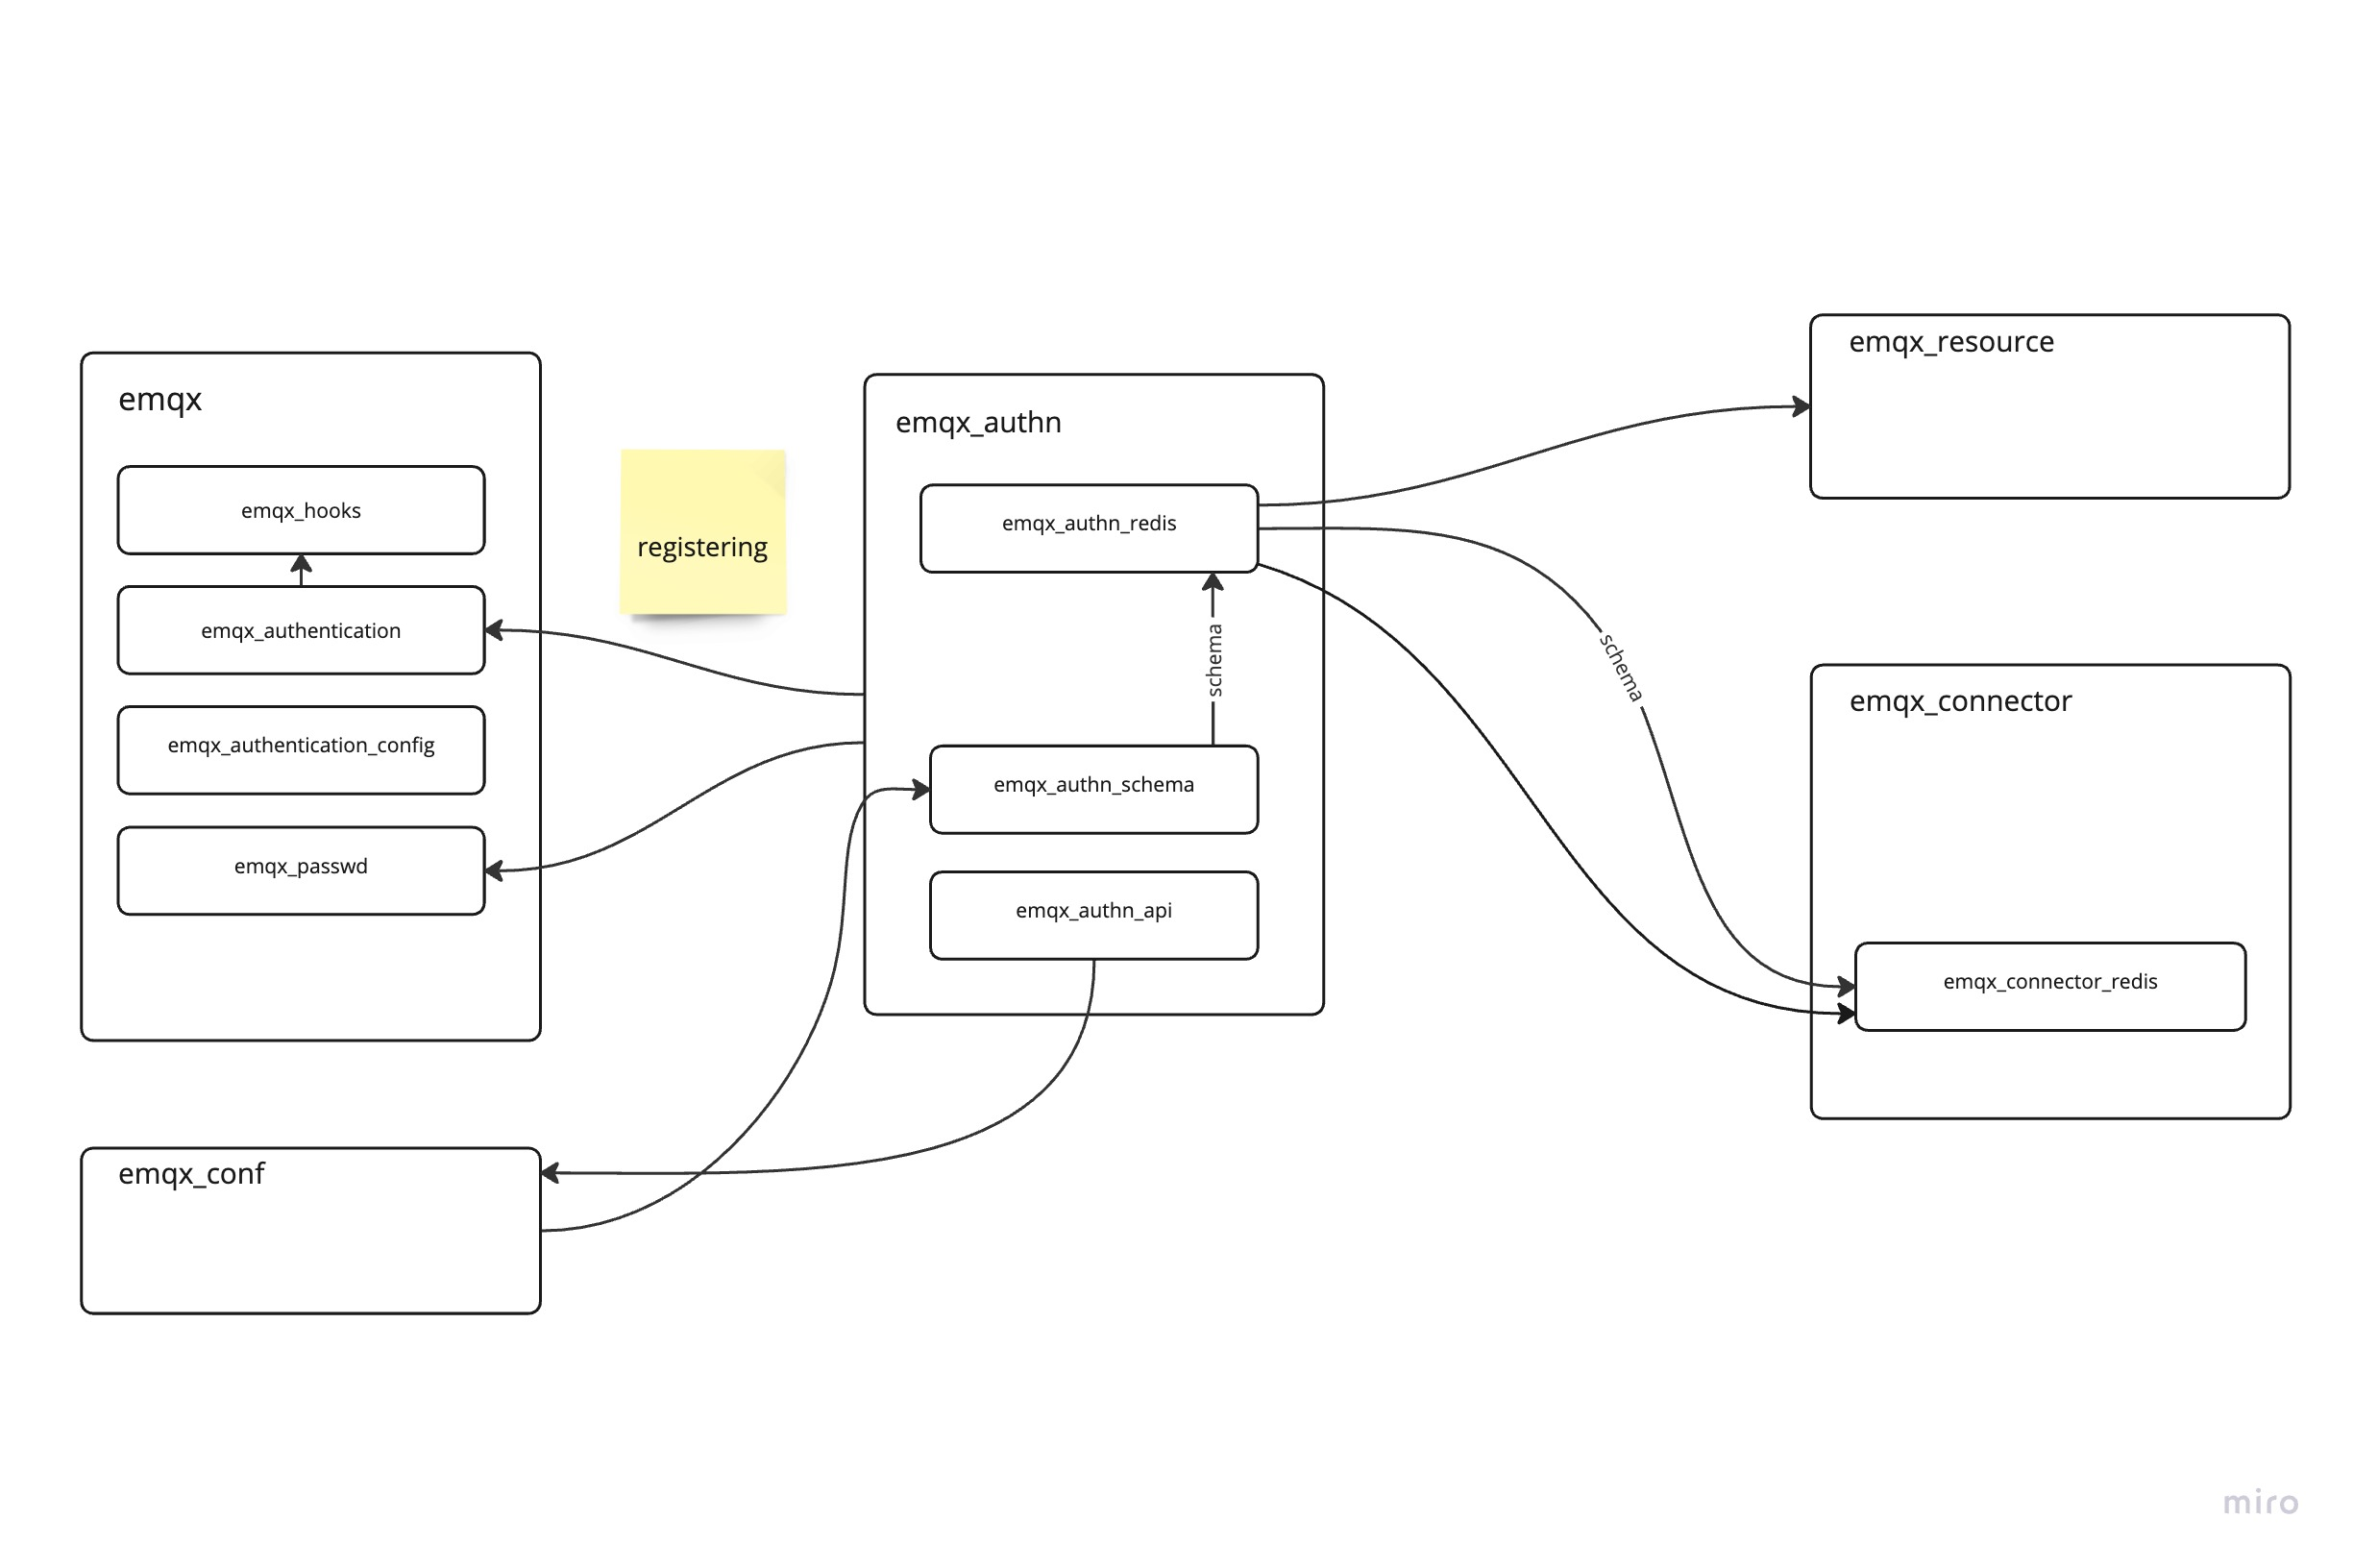
\includegraphics[width=10cm, keepaspectratio]{images/authn-now.jpeg}
    \end{center}
\end{frame}

\begin{frame}
    \frametitle{Auth Refactoring}
    \framesubtitle{Now — issues}

    \begin{center}
        \begin{itemize}
            \item Authn app is actually partially resides inside \lstinline{emqx} app
            \item It is difficult to describe concisely what authn app does
        \end{itemize}
    \end{center}
\end{frame}

\begin{frame}
    \frametitle{Auth Refactoring}
    \framesubtitle{Planned}

    \begin{center}
            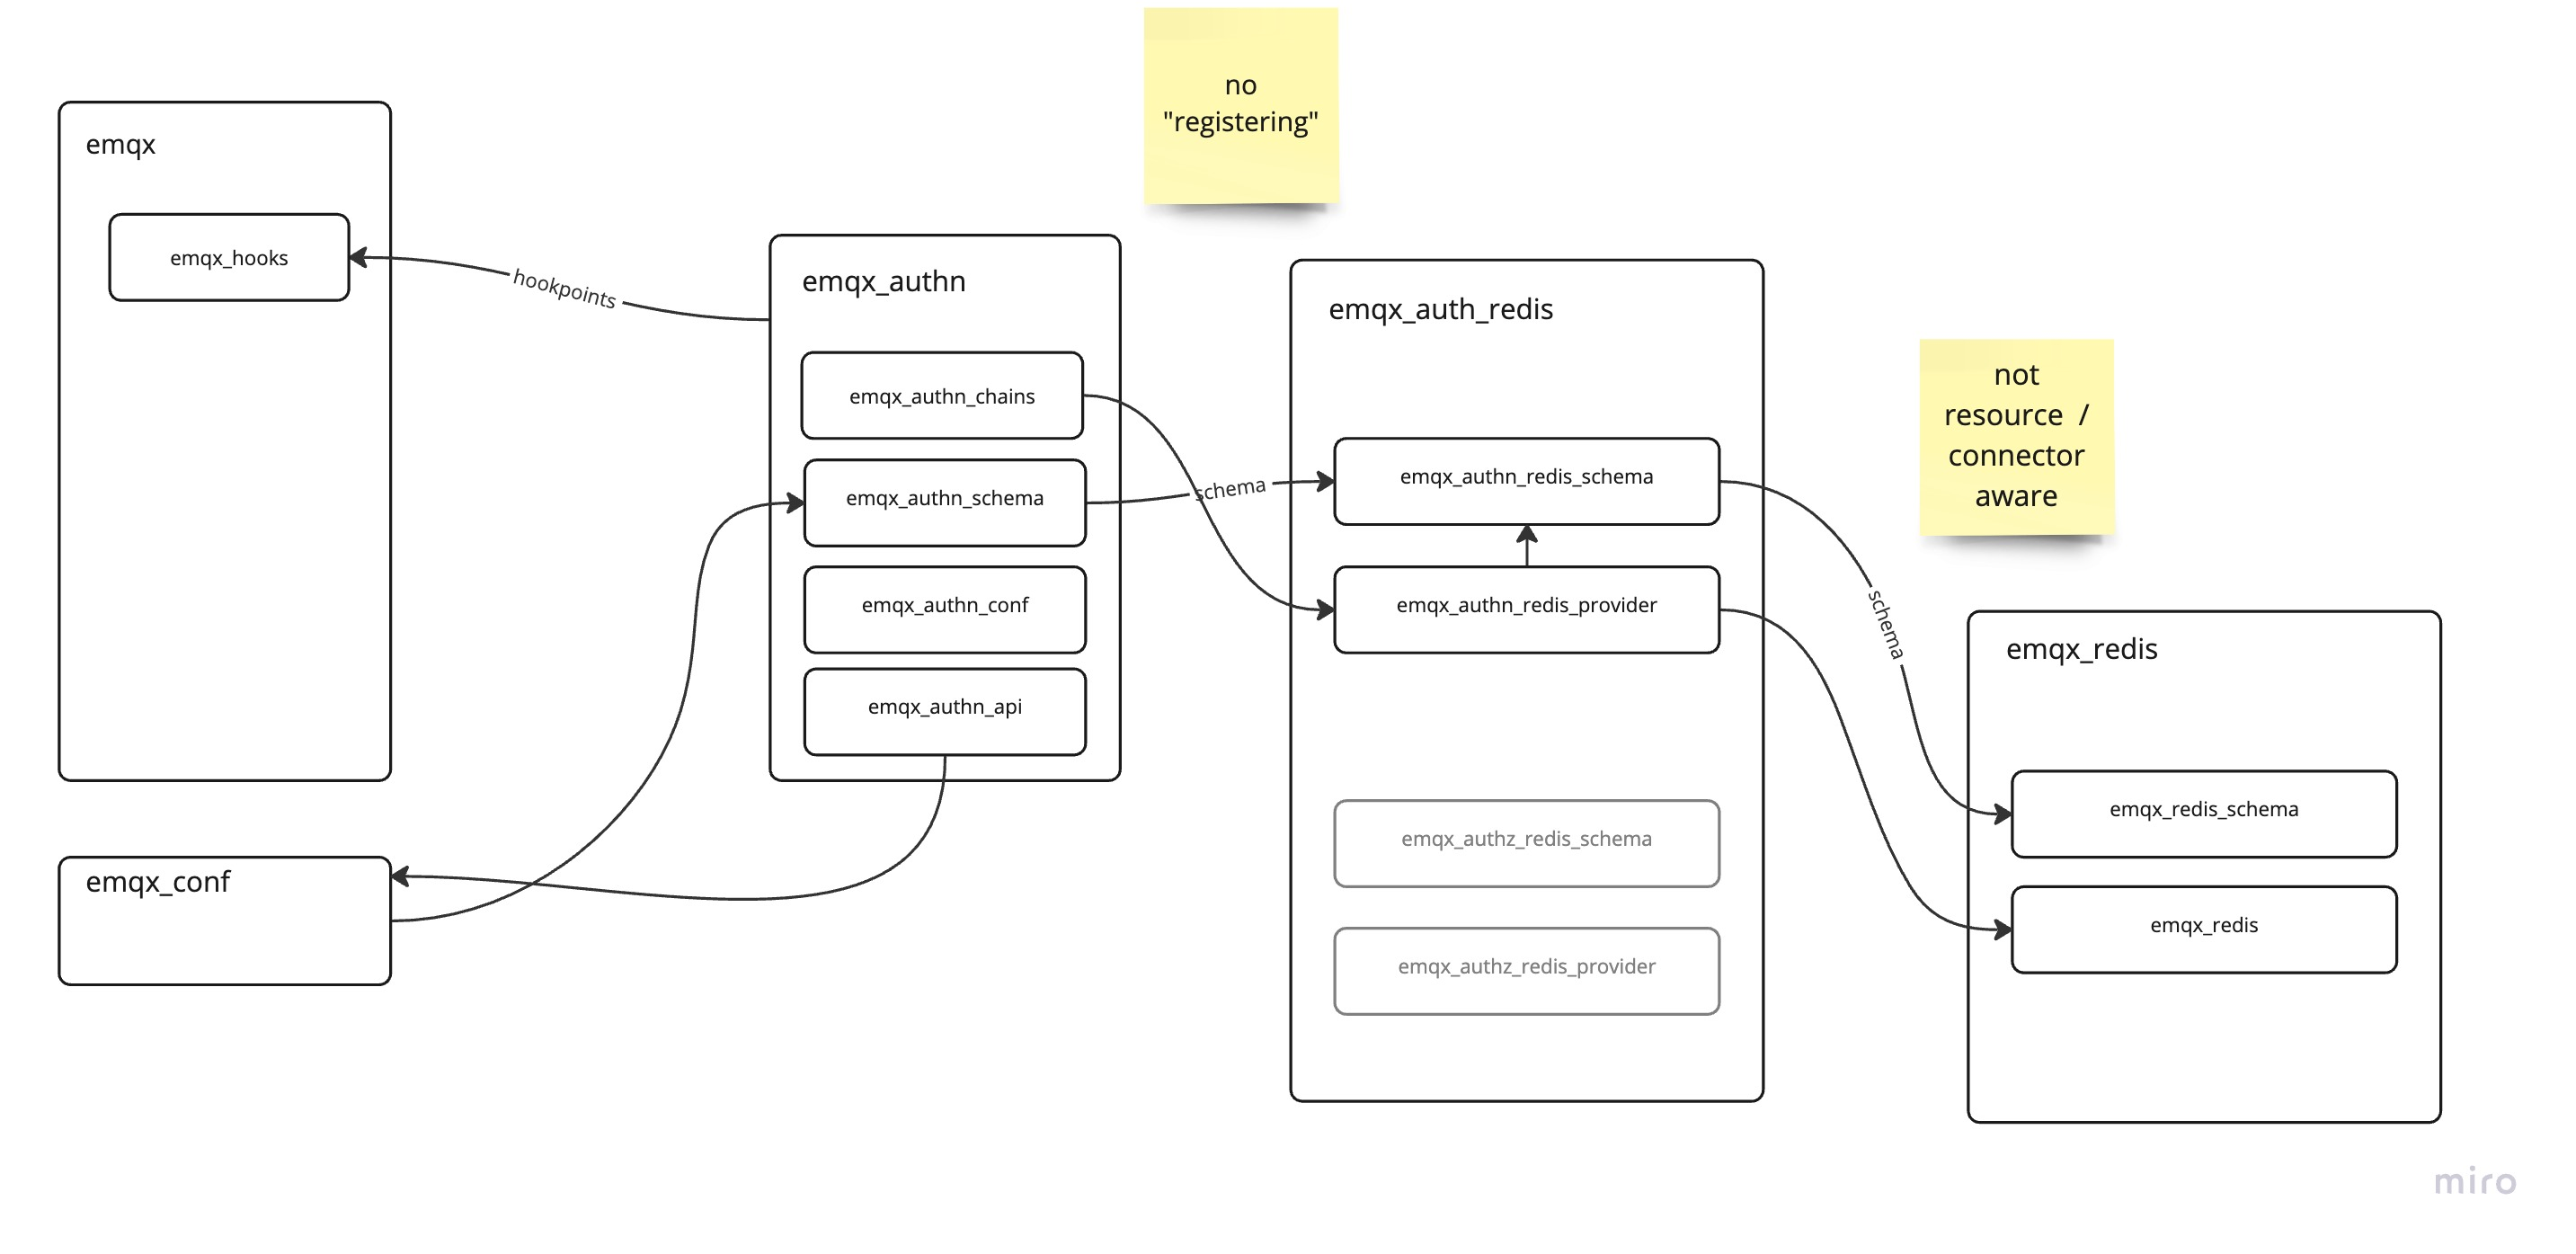
\includegraphics[width=10cm, keepaspectratio]{images/authn-planned.jpeg}
    \end{center}
\end{frame}

\begin{frame}
    \frametitle{Auth Refactoring}
    \framesubtitle{Planned}

    \begin{center}
        \begin{itemize}
            \item Extract authn concerns from \lstinline{emqx} app
            \item *Interact with \lstinline{emqx} only via hooks, as in v4
            \item Extract backend interaction from \lstinline{emqx_authn} app
            \item Remove unnecessary IoC — no authn provider "registration"
        \end{itemize}
    \end{center}
\end{frame}

\begin{frame}
    \frametitle{Auth Refactoring}
    \framesubtitle{Responsibilities}

    \begin{center}
        \begin{itemize}
            \item \lstinline{emqx_authn} app — configuring authantication chains (we may rename it to \lstinline{emqx_authn_chain})
            \item \lstinline{emqx_auth_redis}-like apps — implementing redis backend for authn and authz
        \end{itemize}
    \end{center}
\end{frame}

\begin{frame}
    \begin{center}
        Thank you!
    \end{center}
\end{frame}

\end{document}
